Nonfungible tokens are a whole `class' of digital token, separate and distinct from everything discussed to this point. They are generally \href{https://www.signaturelitigation.com/nfts-recognised-as-property-lavinia-deborah-osbourne-v-1-persons-unknown-2-ozone-networks-inc-trading-as-opensea/}{recognised in law} as property in their own right \cite{moringiello2021property, fairfield2021tokenized}. In the Initial Coin Offering (ICO) and project tokens detailed earlier, and limiting this description to the Ethereum network for now, a project launching an ERC-20 token commits contract code to the blockchain, and this contract then mediates the issuance and management of millions or billions of tokens associated with that project, and it's use case. \href{https://ethereum.org/en/developers/docs/standards/tokens/erc-20/}{ERC-20} is a \href{https://en.wikipedia.org/wiki/Fungibility}{fungible} token issuance. Each of the projects' tokens is interchangeable with any other token. They're all the same from the point of view of the user.\par
Rather than the ERC-20 contract type used for fungible token issuance NTFs predominantly use ERC-721 protocol on Ethereum (just different instructions). It's the case that most NFTs in the 2021/2 hype bubble are algorithmically generated sets of themed art (so called PFP-NFT). Tens of thousands of distinct tokens are `minted', each one being a complex transaction commitment to the Ethereum blockchain, along with it's associated gas fee. These minting events were much hyped social occasions (before the \href{https://www.theguardian.com/technology/2022/jul/02/nft-sales-hit-12-month-low-after-cryptocurrency-crash?}{2022 market crash}), and happened very quickly, with users clamouring to create art with randomly allocated features from the art schema associated with the project. Lucky winners could find themselves with an NFT art piece with more than an average number of `rare' features. If the overall mint becomes more popular, then the secondary market for all of those mints goes up, and because of the liquidity premium they can go up a lot. The perceived rarer mints go up a lot more. This whole process is \href{https://memoakten.medium.com/the-unreasonable-ecological-cost-of-cryptoart-2221d3eb2053}{very energy intensive} on the chain, and the vast majority of these project simply \href{https://www.turing.ac.uk/blog/non-fungible-tokens-can-we-predict-price-theyll-sell}{trend to zero value}. In response to this appalling cost benefit analysis the Ethereum foundation have proposed \href{https://eips.ethereum.org/EIPS/eip-2309}{EIP-2309} to make minting NFTs more efficient. They say ``This standard lets you mint as many as you like in one transaction!''\par
The Ethereum foundation give their somewhat constrained view of \href{https://ethereum.org/en/nft/}{NFTs on their website} and it's a useful primer. On that page they detail some of the use cases, as listed below, with a critique added:
\begin{itemize}
\item Digital content; this is the dominant use case right now. Much more on this later.
\item Gaming items; again more on this later, it's an obvious enough use case but \href{https://climatereplay.org/nfts/nft-digital-ownership-pledge/}{complex politics} in the intersection of games and crypto have stalled the adoption curve.
\item Domain names; this is just starting to reach for applications now, why not a database with the ISP/host?
\item Physical items; seemed like a clear over-reach as transfer of the NFT does not imply transfer of the object, but this is emerging as the growth use case.
\item Investments and collateral; while this was an emergent option in the space, it's likely been a bubble, as owners of the tokens cast around for additional liquidity, and loan businesses chased yield with higher risk. The \href{https://newsletter.banklesshq.com/p/three-arrows-capital-grayscale-maker-lido}{recent implosion} of lenders and funds in the crypto space was partly a function of supposedly world class risk managers accepting jpegs as collateral.
\end{itemize}
Moving away from Ethereum, NFTs can be minted on most of the other level one chains. Solana is a great newcomer example. Sol is a terrible chain with regards to decentralisation, but thanks to that it's far cheaper and faster to mint NFTs on it, and it was becoming a \href{https://markets.businessinsider.com/news/currencies/ethereum-eth-killers-nfts-defi-solana-cardano-wax-crypto-investing-2022-1}{troubling competitor} for Eth before the FTX ponzi scheme collapse destroyed it's market value (Figure \ref{fig:solnfts}).\par 
\begin{figure*}[ht]\centering % Using \begin{figure*} makes the figure take up the entire width of the page
	\includegraphics[width=0.7\linewidth]{solnfts}
	\caption{Solana NFT markets are enjoying growth compared to Opensea on Ethereum, even in the downturn.}
	\label{fig:solnfts}
\end{figure*}
The same might be true for Cardano's ADA, though ADA is struggling to hold onto it's market position despite some technical advances. It's worth reiterating here that the nature of these digital tools likely makes for a `winner take all' market dynamic over time. With fees being central to this generative NFT use case it's possible to see that highly centralised, fast, and cheap chains will capture and eventually dominate the space. Remember that this likely (game theoretic) outcome might as well be a database running without the stark inefficiencies of blockchain. The whole NFT space is a gamble on consumer enthusiasm for spending money continuing to outpace logic.\par 
Astonishingly, according to a JPMorgan insider market report (\href{https://www.coindesk.com/podcasts/the-breakdown-with-nlw/jpmorgan-bitcoin-shows-some-merit-as-a-store-of-value/}{reported on in a podcast}), only around 2 million people have ever actually interacted with NFTs. One analysis suggests that a single entity accounts for 3 of the top 4 holders, having made 32,000 ETH from the NFT boom. This suggests heavy market manipulation and is far from the egalitarian landscape claimed in the hype. Tellingly it's thought around \href{https://uk.finance.yahoo.com/news/three-arrows-wanted-100m-nft-161811450.html}{10\% of the trading volume} on market leading platform `Super Rare' was by the now bankrupt venture capital firm `Three Arrows'. \par
With that said NFTs have clearly allowed \href{https://en.wikipedia.org/wiki/List_of_most_expensive_non-fungible_tokens}{digital and new media artists} to connect with audiences without gatekeepers. Established mediators and curators of art have been caught totally wrongfooted, and NFTs seem to give a way for them to be cut out completely. There are suggestions of applications beyond this initial digital art scope. This is a compounding, and disrupting paradigm change.\par
%Users of NFT markets have \href{https://blog.chainalysis.com/reports/nft-market-report-preview-2021/}{injected around \$30 billion into the tokens during 2021}. 
\section{Key use cases}

\subsection{Art}
The recent surge of interest in NFT's during early 2021 has largely been
driven by digital art NFT's, despite the origins of digital art NFT's
started much earlier in 2014. New York artist \href{https://www.mccoyspace.com/project/125/}{Kevin McCoy's
\emph{Quantum}} is widely recognised as the first piece of art created
as an NFT. However it was during early 2021 that art NFT's started to
gain significant attention; by the end of 2021, nearly \href{https://www.paymentscardsandmobile.com/state-of-the-blockchain-nfts-explode-onto-scene-in-2021/}{£31b
had been spent} on NFT purchases, a considerable and exponential growth
given \href{https://raritysniper.com/news/nfts-exploded-in-2021-with-25-billion-in-sales/}{2020
sales of \textasciitilde£71m}
High profile digital artists such as \emph{Beeple} whose
\href{https://www.forbes.com/sites/abrambrown/2021/03/11/beeple-art-sells-for-693-million-becoming-most-expensive-nft-ever/?sh=3f237d1c2448}{recent
recording break sale} of his NFT \emph{``The first 5000 days''} (Figure \ref{fig:first5000days}) at Christies (a long established British auction house,
specialising in high profile precious work of art) for £52.9m helped
bring NFT's into the public spotlight and wider give them global
attention.

\begin{figure*}[ht]\centering % Using \begin{figure*} makes the figure take up the entire width of the page
	\includegraphics[width=\linewidth]{first5000days}
	\caption{Beeple: First 5000 days, \href{https://onlineonly.christies.com/s/beeple-first-5000-days/lots/2020}{taken from the Christies website, assumed fair use}.}
	\label{fig:first5000days}
\end{figure*}

Art as NFT's offer the following advantages:

\subsubsection{Immutable Nominal Authenticity} 
Art fraud such as false
  representation, forgeries, plagiarism have been a reoccurring blight
  since art has existed; artists and works of art have been open to
  abuse by forgers, black market profiteers and even fellow artists
  laying claim to works of art of others. Unless a work of art is sold,
  exhibited or listed, documenting when and who created it, the
  \emph{nominal authenticity,} which Dutton states as the
  \emph{``correct identification of the origins, authorship, or
  provenance of an object''} \cite{dutton2003authenticity} can be increasingly mutable over a period
  of time, dependent on a multitude of factors, including; the artists
  existing profile, how widely and where the work of art is exhibited,
  if the work of art is commissioned by a patron, if it's sold, and
  profile of the buyer/collector. At its most basic level, once a work
  of art is `minted' as an NFT (publishing the art work as a unique
  token on the blockchain) this functions as an immutable publicly
  accessible proof of ownership and by extension proof of creation. The
  act of minting is not purely limited to digital art; all an artist
  requires is a digital representation of any physical art (sculpture,
  physical painting, installation etc..) which can be used as a proxy
  allowing artists to record the date of creation/origin of a physical
  piece of art on the blockchain, a buyer purchasing the NFT can be
  provided the actual physical artwork as part of the NFT. Nominal
  authenticity becomes secure and immutable for the lifetime of the blockchain (by no means assured).

\subsubsection{Secure Digital Provenance}
\href{https://en.wikipedia.org/wiki/Provenance}{Provenance} (or the chain of custody) is an important aspect in works of art, antiques and antiquities. Provenance not only helps assign work to an artist but also documents ownership history. Digital provenance, an inherent feature of NFT's means provenance now no longer becomes what has historically sometime been a contentious detective's game at the best of times; one that is open to fraud, misinterpretation and entirely reliant on good record keeping.\par
Since provenance can contribute to the value of a piece of art (benefiting both the creator and collector) the use of the blockchain as an open, secure ledger is a far more trustworthy system than traditional methods of artistic provenance that were cobbled together; often
consisting of a mix of physical and digital documents spanning private
\& public sale receipts, art/museum gallery exhibitions and private
record keeping). Digital provenance provided when an artist `mints' a
piece of art into an NFT allows artists and collectors to record a
secure, permanent unalterable history of transactions for a specific
piece of art, providing future collector complete trust in the origin
and custody of a piece of art.
\subsubsection{Decentralised automated royalty payments} 
Traditionally if a  piece of art is sold, the first sale may (but not always) benefit the
  artist financially, however secondary and any subsequent sales would
  only ever financially benefit the buyer/collector; the original artist
  would rarely benefit. However If a work of art is minted into an NFT,
  royalty payments can be predetermined and automated in perpetuity
  directly by the use of a `smart contract'. Smart contracts are small,
  automated scripts/programs that run automatically and independently of
  a buyer/seller; pre-determined conditions are set by the buyer; these
  trigger when certain conditions are met i.e. These cannot yet be enforced ``on chain'' and the NFT auction houses online have engaged in a race to the bottom and stopped enforcing royalty payments through their systems. This element might not even be possible, though there is some hope that we could enable this in the complex logic offered by the RGB protocol.
\subsubsection{On sale transfer}
20\% of total sale amount into digital wallet of the creator.
80\% of total sale amount into digital wallet of the seller.

Once the royalty payment rate is set by the artist/creator, future
royalties of all sales can be paid directly to the artist/creator
account (via a digital wallet) without the need of a third party
(traditionally a gallery/agent etc..).

Smart contract driven NFT's means that even if piece of art is resold 5,
10 or even a 100,000 times moving through 5, 10 or even a 100,000
different collectors; a pre-determined royalty payment rate set by the
creator would still guarantee the artist/creator is paid directly from
each and every future sale.

Historically provenance for works of art may span across generations,
for instance Gabriël Metsu's oil on canvas painting \emph{The Lace
Maker's} provenance, first recorded in 1722, now spans 300 years of
ownership, including from a British Baron in the 19\textsuperscript{th}
century to an American philanthropist in the 20\textsuperscript{th}
century.) Metsu died young at the age of 38, leaving a widow; neither
his/her relatives/descendants benefit from his original work, 300 years
later this would be near impossible to facilitate with traditional
systems, as even legal contracts are open and prone to the ravages of
time.

NFT smart contracts hold an incredibly potential; an artists descendants
financially benefiting directly from the resale of a piece of work long
after the artist/museum's/gallery or even state have turned to dust as
long as the original creator's digital wallet is accessible, \emph{the
blockhain becomes an everlasting digital patron} ensuring


NFT art currently suffers from the same failure of decentralisation already discussed in the Ethererum technology stack, but this is compounded by the normalisation of intermediate art brokers \href{https://moxie.org/2022/01/07/web3-first-impressions.html}{continuing to custody} the NFTs even after sale. They are usually selling a pointer to their own servers. The market is nascent and evolving, but it's currently not delivering on it's core promise.\par
Proof of ownership is intuitively a pretty obvious application for the technology, but again it's hard to justify the expense when the benefits are so slim. \href{https://www.bullishlybred.com/}{Bulldogs on the blockchain} is a clear gimmick, and might even incentivise poor behaviours as there are two products here which are not necessarily aligned. Much has been written over the years about \href{https://propy.com/browse/propy-nft/}{deeds to property} being passed through blockchains, cutting out the middle man, but in the event that a house deed NFT was hacked and stolen it's obviously not the case that the property would then pass to the hacker.\par 
One of the most interesting companies is Yuga Labs, who launched the incredibly popular Bored Ape Yacht club set of 10,000 algorithmically generated NFTs. These Ethereum based NFTs were based loosely on the `Crypto Punks' model of PFP-NFT (variously profile picture project, picture for proof, and picture for profile - no definition remains uncontested for long). Yuga launched with a better commercialisation model for the holders, and a strong marketing drive into celebrity circles. They now regularly change hands for hundreds of thousands of pounds. Even this `blue chip' NFT is not without \href{https://twitter.com/coryklippsten/status/1538909505236283392}{serious criticism}: \textit{``I'd put it at 99.99\% the project is in fact a deliberate troll, intentionally replete with Nazi symbols and esoteric racist dog whistles''}\par
Yuga recently bought the artistic rights to the commercial reuse of similarly popular (and preceding) Punks set. This is interesting because they have again handed the commercial re-use rights to the owners of the individual NFTs. This raises the same \href{https://www.bloomberg.com/news/articles/2022-03-21/bored-ape-nft-spinoff-venture-gone-sour-sparks-legal-fight}{confusing problem} with attaching commercial rights to an easily stolen token as NFTs for real estate does. This has been demonstrated recently when Seth Green had a Bored Ape stolen after \href{https://www.buzzfeednews.com/article/sarahemerson/seth-green-bored-ape-stolen-tv-show}{creating an animated show around it's IP}. Many more contradictions and ambiguities in NFT licenses are emerging. Galaxy Digital have \href{https://www.galaxy.com/research/insights/a-survey-of-nft-licenses-facts-and-fictions/}{surveyed the landscape}:
\textit{``Contrary to the ethos of Web3, NFTs today convey exactly zero ownership rights for the underlying artwork to their token holders. Instead, the arrangements between NFT issuers and token holders resemble a distinctly Web2 maze of opaque, misleading, complex, and restrictive licensing agreements, and popular secondary markets like OpenSea provide no material disclosures regarding these arrangements to purchasers. Something more is required, and that `something' is a legal agreement between the owner of the image—known as the `copyright holder' and the NFT holder specifying what rights the NFT holder has with respect to the image. To the extent an NFT purchaser has any rights to the image associated with his or her NFT at all, those rights flow not from his or her ownership of the token, but from the terms and conditions contained in the license issued by the NFT Project governing the NFT holder’s purchase and use of the image. Accordingly, for the vast majority of NFT projects, owning the NFT does not mean you own the corresponding digital content that is displayed when you sync your wallet to OpenSea. That content, as it turns out, is owned and retained by the owner of the copyright associated with that digital content, typically the NFT project.
After reviewing the most used license agreements for NFT projects, it becomes apparent that NFT standards and smart contracts do not recognize off-chain law.''} There may already be a response from the industry to this in the shape of \href{https://a16zcrypto.com/introducing-nft-licenses/}{a16z's ``can't be evil'' license proposal}.\par
Even so, the community around these collections is incredibly strong, mixing developers, artists, the rich and famous, and the fortunate and early, into a cohesive community who communicate online. The developer `good will' is enormous, and it seems possible that this will lead to faster and broader innovation around the collections, and out into \href{https://twitter.com/yugalabs/status/1505014986556551172?}{metaverse applications}. The brand is strong, and the individual NFT items both benefit from, and reinforce that brand, while adding personal narratives and human interest.\par 
As a gauge of how frothy this market still is it's interesting to look at the APE token which Yuga just launched. They airdropped 10,000 of the tokens free to each of the 10,000 NFT holders. This instantly created a multi-billion dollar market cap, and a top 50 `crypto' out of thin air, based purely on their brand. It's clear that there is both brand, and a market here.\par
A recent report from "Base Layer" tries to capture the community `feature' of big brand NFTs. \href{https://baselayer.so/crypto-culture-decoded}{``Crypto culture decoded''} explains that is is these online communities which are the attraction not necessarily the art. This is a powerful `in group' argument, though speculation remains the most likely underpinning.\par

%\href{https://amycastor.com/2021/03/14/metakovan-the-mystery-beeple-art-buyer-and-his-nft-defi-scheme/}{Beeple scam}

While it is likely that this is currently a speculative bubble, that is \href{https://www.bbc.co.uk/news/business-61102759}{waning already} (Figure \ref{fig:monkey}), it seems certain that the technology is here to stay in some form.\par

\begin{figure*}[ht]\centering % Using \begin{figure*} makes the figure take up the entire width of the page
	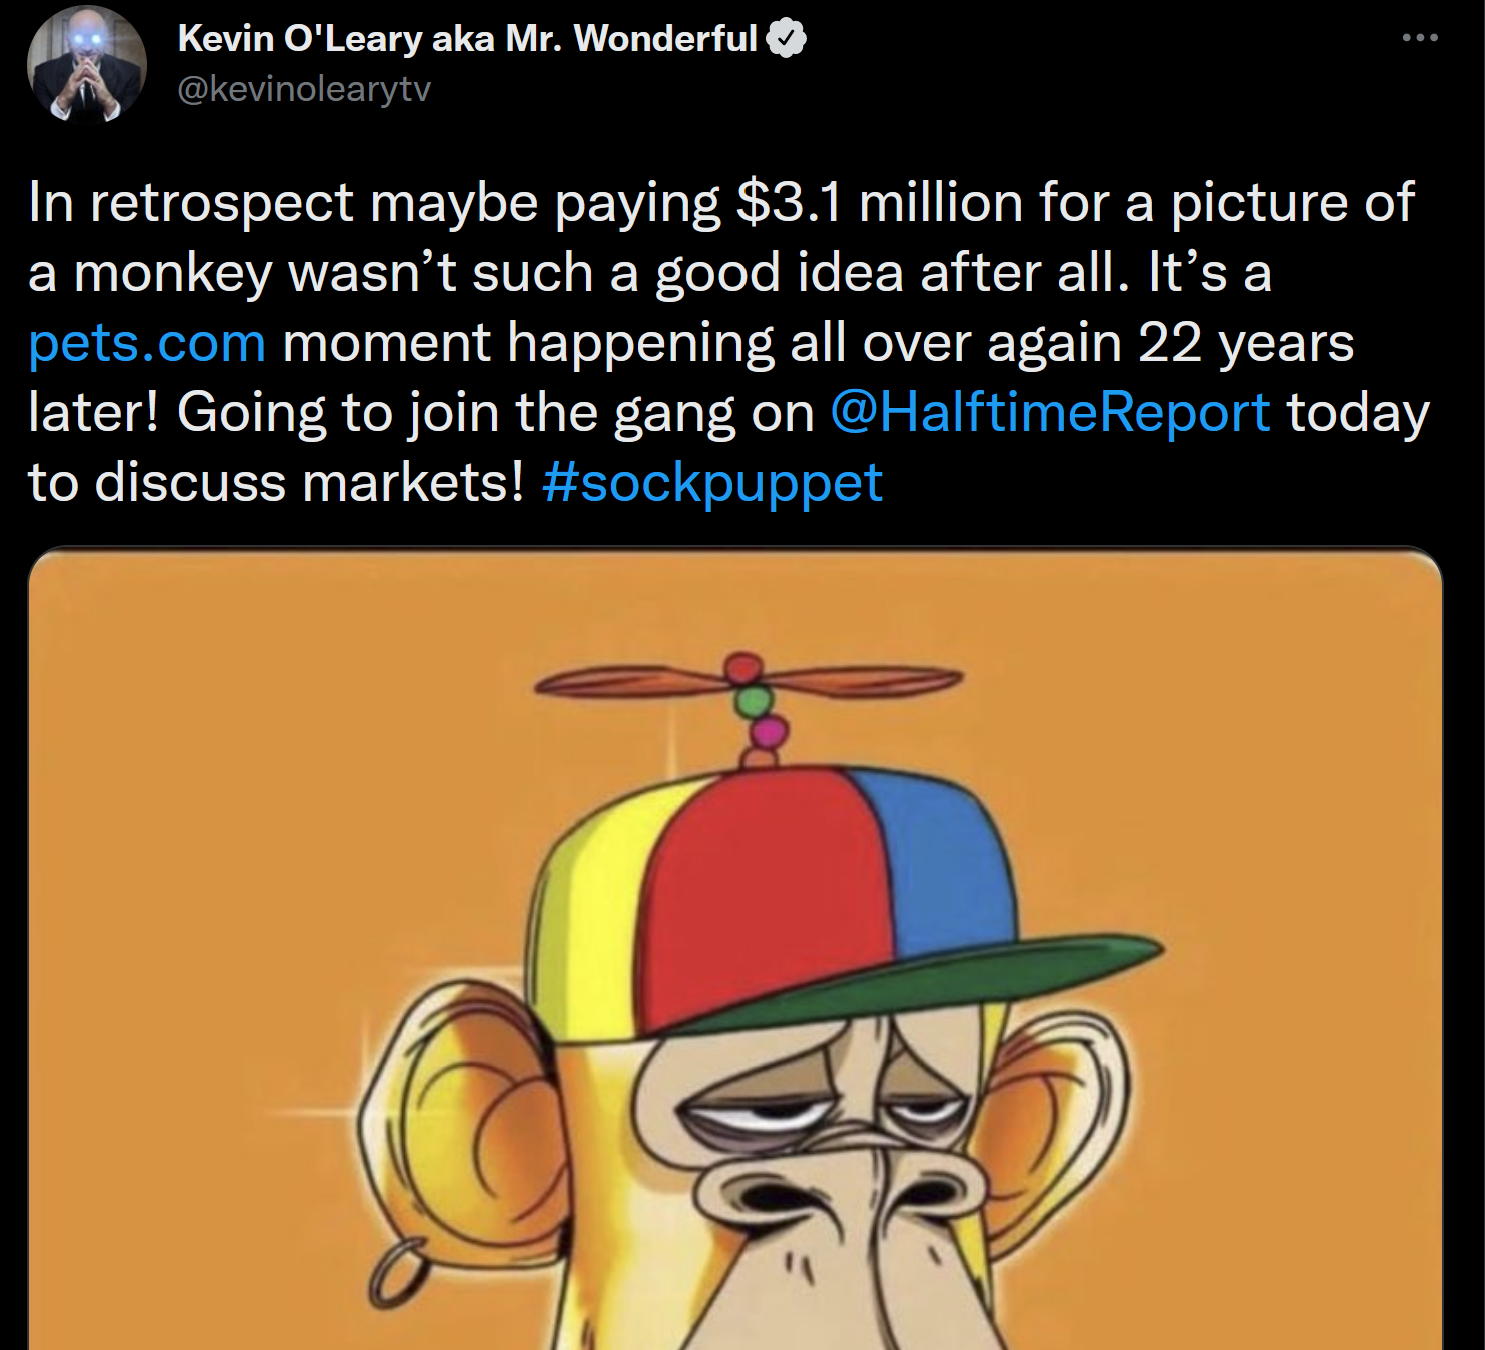
\includegraphics[width=\linewidth]{monkey}
	\caption{The \href{https://www.coingecko.com/en/nft/bored-ape-yacht-club}{bubble bursts} on Yuga Bored Apes for now.}
	\label{fig:monkey}
\end{figure*}


\subsection{Computer \& Video Games}
Computer \& Video games are a huge global business, exponential global
growth over the last 30 years has seen this grow to a point where it has
eclipsed both the
\href{https://www.businessinsider.com/video-game-industry-revenues-exceed-sports-and-film-combined-idc-2020-12?r=US\&IR=T}{global
movie and North American sports industries} combined.

A global industry with revenues over £120b,
\href{https://www.wepc.com/news/video-game-statistics/}{with
\textasciitilde half the people on the planet} playing some form of
games in 2021.

As the games industry has evolved and matured over the last 40 years,
secondary markets have emerged, most notably the `second hand' games
resale market. The rise of `retro' gaming, has demonstrated the second
hand market is a lucrative one for private resellers, an unopened copy
of Super Mario Bros for the Nintendo Entertainment System
\href{https://www.nytimes.com/2021/08/06/business/super-mario-bros-sale-record.html}{recently
selling for £1.5M} to the extent the market has seen
\href{https://www.businessinsider.com/retro-gaming-market-being-overtaken-by-speculators-2021-9?r=US\&IR=T}{speculators
looking to cash in} on the huge global interest in retro/second hand
games.\par
Despite publishers and developers increasingly moving to non-physical
digital only' games, the demand for used games remains incredibly high.\par
Whilst some retailers have adapted their business models to include reselling of retro/second hand games, the vast majority of publisher/developers/retailers aren't able to directly benefit from the
emerging retro/second hand games market. The potential of \emph{video
games as NFT's} presents a huge opportunity for publishers, developers
and players alike, offering the following advantages:
\subsubsection{Royalty Sales on Pre-owned Games} ; A predetermined proportion
  of any resale of a used game can automated in perpetuity via smart
  contracts; once these are set by the publisher, future royalties of
  all sales can be paid directly to the publishers/developers wallets (a
  digital account) without the need of a third party (traditionally a
  retail entity). Traditionally only the initial first sale of a game
  would financially benefit the publisher/developer/retailer, secondary
  and subsequent sales would only ever financially benefit the
  purchaser, with many developers/publishers arguing this is hurting the
  wider industry through the loss of significant income generated by the
  secondary and subsequent sales, sometimes over the course of decades.
  However the use of NFT's smart contracts means that if a game is
  sold/resold through 10,000 collectors; a pre-determined royalty
  payment rate set by the publisher would still guarantee the publisher
  (and or developer/retailer) takes a proportion of any future sales.
\subsubsection{Monetisation of User Generated Content:} Games as a NFT's
  offer ability to monetise UGC: User generated content. Video games such as
\href{https://www.businessofapps.com/data/pokemon-go-statistics/}{Nintendo's
\emph{Pokemon Go}} \emph{(166 million players)},
\href{https://techacake.com/destiny-2-player-count/\#:~:text=The\%20total\%20player\%20base\%20of,to\%20be\%2038\%20million\%20players.\&text=According\%20to\%20the\%20source\%2C\%20the,in\%20terms\%20of\%20player\%20population.}{Bungie's
\emph{Destiny 2}} \emph{(38 million players)} or
\href{https://fictionhorizon.com/how-many-people-play-genshin-impact/\#:~:text=Genshin\%20Impact\%20had\%20approximately\%209,million\%20users\%20in\%20June\%202021.}{miHoYo's
Genshin Impact} (\emph{9 million players} ) all have large, established
and significant player bases. What is noteworthy, the games are designed
to encourage players may spend hundreds, or in some cases thousands of
hours on one game alone; according to
\href{https://destinytracker.com/destiny/leaderboards/all/minutesplayedtotal?grouped=true\&page=1}{Destinytracker.com},
the top players have amassed total play times over 20,000 hours, close
to 1,000 days or \textasciitilde{} 3 years, which is incredible feat
given Destiny 2 only launched 5 years ago in 2017.\par
Destiny/Pokemon Go and Genshin Impact revolve around a central key game
mechanic; players investing significant amounts of time collecting in
game digital assets; characters/weapons/items, often classed as `rare'
or `exotic' or `5 Star'. These collectibles usually found by a
combination of the accrual of in-game time, completing quests,
purchasing additional in-game items/boosters, and luck (`RNG'). Players
are often encouraged to share their collections of rare
characters/weapons/ objects through in-game achievements, triumphs,
scores acting as a mark of distinction/status symbol.\par
Traditionally there has been nothing that went beyond sharing the
\emph{digital badge} (i.e triumph/achievement/accomplishment) on a on
social media/gamer's platform profile. However NFT's offer the ideal
system for developers/publishers and even players to monetise user
generated/customised data (such as a players unique save game data), simultaneously allowing:
a) creation of an additional monetised ecosystem to meet player demands
i.e. some players who are willing to monetise and `sell' their invested
time in a particular product/service to other players with little time
but willing to pay other players for `grinding' (progressing laborious
in game tasks) and a more advanced in-game progression point.
The potential to provide publishers/developers with an additional
long-term income stream, providing a better ROI on computer \& video
game development, which in many instances can cost hundreds of millions
in development costs spanning 5/10 years, is undeniable.
\subsubsection{Play to earn revenue models}
This is morally dicey at this time and early startups like \href{https://www.bloomberg.com/news/features/2022-06-10/axie-infinity-axs-crypto-game-promised-nft-riches-gave-ruin}{Axie Infinity are in serious trouble}. A (long) \href{https://www.youtube.com/watch?v=YQ_xWvX1n9g}{video by Dan Olsen} highlights the structural problems with both play to earn and NFTs. On chain analysis suggested that 40\% of accounts in 200 current Web3 games \href{https://gallery.usejigger.com/}{are bots}. 
\subsubsection{Monetizing In game collectibles}
customisable in game assets (vanity
  items such as cosmetic character skins/clothing or collectible items
  that offer player advantages(new weapons/vehicles/mods etc,..)



Traditional gamers have pushed back on the seemingly useful idea of integrating NTFs with traditional games. This may be in part because Ethereum mining has kept graphics card prices high for a decade.

\href{https://www.prnewswire.com/news-releases/hbar-foundation-and-ubisoft-partner-to-support-growth-of-gaming-on-hedera-network-301474971.html}{HBAR partnerships}\par
\href{https://finance.yahoo.com/news/epic-games-vp-people-have-lost-interest-in-the-metaverse-200725562.html}{Critique from Marc Petit of Epic and Unreal}.\par
The \href{https://twitter.com/justinkan/status/1491270239967154178}{following text} is from Justin Kan, co-founder of twitch: \textit{``NFTs are a better business model for games. Many gamers seem to be raging hard against game studios selling NFTs. But NFTs are also better for players. Here’s why I think blockchain games will be the predominant business model in gaming in ten years. NFTs are a better business model for funding games . Example: recently I invested in a new web3 game SynCityHQ. They are building a mafia metaverse and raised \$3M in their initial NFT drop.\\ NFTs give studios access to a new capital market for raising capital from the crowd.NFTs can be a better ongoing model for games. Web3 games will open economies, and by building the games on open and programmable assets (tokens + NFTs) they will create far more economic value than they could from any one game. Imagine Fortnite, but other developers can build experiences on top of the V-Bucks and skins. Epic would get a royalty every time any transaction happens. As big as Fortnite is today, Open Fortnite could be much bigger, because it will be a true platform. NFTs are better for gamers Allowing gamers to have ownership of the assets they buy and earn in game allows them to participate in the potential growth of a game. It lets gamers preserve some economic value when they switch to playing something new. But what about the criticisms of NFTs?\\
Here are my thoughts on the common FUDs: "It’s just a money grab on the part of the studios!"\\
Game studios already switched over to the model of selling in-game items, cosmetics, etc to players long ago. But currently the digital stuff players are buying isn’t re-sellable. NFT ownership is strictly better for players. "The games aren’t real games." This reminds me of the criticism of free-to-play in 2008, when the games were Mafia Wars / FarmVille. We haven’t had time for great developers to create incredible experiences yet. Everyone investing in games knows there are great teams building. "Game NFTs aren’t really decentralized because they rely on models / assets inside centralized game clients."
Crypto is as much a movement as it is a technology. Putting items on a blockchain is what gives people trust that they have participatory ownership...which make people willing to buy in to the game. These assets are “backed” by blockchain.
The fact that these item collections are NFTs will make other people willing to build on top of them. "NFTs are bad for the environment." Solana and L2s solve this. NFT games are better for players and for game developers. Like the free-to-play revolution changed gaming, so will blockchain. The games of the future will be fully robust, with open and programmable economies.}''
\section{Broader and metaverse uses}
So far according to a16z NFTs break down into:
\begin{itemize}
\item Profile pictures: These were discussed at the start of the chapter and have felt ubiquitous on Twitter over the last couple of years. The major projects will likely hold value, but the hype cycle will likely lead to all profile NFTs going in and out of fashion. There's potentially a fresh wave of this same kind of low key identity hype possible in the metaverse, and indeed the two plausible both intersect and converge.
\item Art and Music: Art has also been discussed above. Peter Thiel, the billionaire venture capitalist who founded PayPal has invested in expanded NTF use cases. The first is `Royal' which is experimentally \href{https://royal.io/}{selling limited NFT tokens} which contractually entitle the holder to a portion of music artist royalties. Spotify are experimenting with music NFTs (and of course in the metaverse). This is an early adopter area, and again likely converges with our planned uses cases as more complex tooling appears. For instance Tim Exile of \href{https://endlesss.fm/}{Endless.fm} talks about digital assets extending to the building blocks of co-created music, and wished to build a music creator economy which distributes value to creators at the instant of the final value transaction with the consumer.
\item Gaming: As discussed there's pushback from the gaming community, but huge investment from the likes of Lego, Blizzard, Epic, Ubisoft etc.
\item Gig tickets: Not only the straightforward use of \href{https://news.yahoo.com/psg-sells-us-220-000-030927515.html}{transferable tickets for events} as NFTs on a blockchain (which is impossible due to the cost right now) but also onward monetisation of ticket stubs as memorabilia. The NBA is \href{https://deadspin.com/investing-in-nft-ticket-stubs-is-likely-one-of-the-nba-1848991991}{already looking at this}.\\
\textit{``The team sells the ticket for face value many many years ago, but when that stub is being sold now for much more many times over, the team gets none of that money,'' York explained. ``But with an NFT stub that changes. Let’s say a new rookie enters the NBA next season and he turns out to be the next LeBron James. That ticket stub from his first game, as an NFT, the team can put a commission on it — 20 percent or however much, the NBA decides that. In 10 years when it’s worth a lot of money, I or whoever owns that NFT, can sell it for say \$100,000. The NBA can still collect 20 percent of that sale, because it’s all on a smart contract.''}\par
It seems so obvious that this will extend to the virtual events space in the metaverse.
\item Utility: These are broadly `membership' style tokens, and this seems like a sensible fit. Peter Thiel (again) for instance launches a \href{https://www.ztonft.com/}{political funding NFT} from Blake Masters to support his senate ambitions. To be clear, Thiel is a fundamentalist libertarian, and at the very least \href{https://gizmodo.com/peter-thiel-bitcoin-talk-miami-2022-1848764790}{highly eccentric}. This is not necessarily a positive for the technology.
\item Virtual worlds are a huge application for NFTs, and this seems like it would be a natural fit for out metaverse application. In reality the \$2B of sold so far is mostly `allocations' in nascent ecosystems, being sold as highly speculative assets, without even a metaverse to use. The majority of that amount is the hyped `Otherland' plots sold under the Bored Apes brand.
\item ``Full stack'' luxury brands. \href{https://medium.com/@nic__carter/redeem-and-retain-nfts-are-the-future-of-luxury-goods-760f00dbce23}{Nic Carter describes} a mating of physical and virtual luxury goods. His is a useful article on the future direction, and he has also \href{https://medium.com/@nic__carter/why-nfts-are-hard-to-explain-48f0ab0a35bf}{provided a primer on NFTs}. There are many such examples already, such as \href{https://nft.tiffany.com/faq/}{Tiffanys `NFTiff' - cryptopunks} collaboration which will automatically generate royalties for Tiffanys and parent company Louis Vitton in perpetuity. Such products prove provenance, create new aftermarket opportunities, and unlock metaverse applications.
\end{itemize}
It is completely reasonable to assert that these use cases could be accomplished without the use of NFT technology, and is part of the hype bubble.\par
Twitter user Cantino.Eth offers an exhaustive roundup of what they think future uses might be. It's a \href{https://twitter.com/chriscantino/status/1542930648750608387}{thread full of industry insider jargon} but it's indicative of a shift in focus from speculation to `building' as the market conditions change. Some of the more interesting (less arcane) use cases identified in the thread are summarised very briefly below, again with comments as to how this might pertain to our metaverse applications.
\begin{itemize}
\item Hobby tokens, demonstrating interest in an activity. This is potentially a metaverse adaptation of badges on a blazer in the real world, and might serve to drive communities in a metaverse. The same is true for activism and political alighnment. It's a great idea and worth developing.
\item Professional Networks and qualification badges, like a LinkedIn qualification panel, but in the metaverse. A cisco NFT in the metaverse for a CCNA qualification makes intuitive sense. 
\item Badges to indicate membership of distributed projects within a metaverse. This allows users to identify avatars with shared goals in the metaverse.
\item Retail incentives, like brand loyalty stamps or rewards for participation in marketing, or early access programmes. This is a true in a metaverse marketplace as it is in a real world coffee shop.
\item Multiplayer communities with incentives to hit collective milestones. ``Collecting as a team sport''. This again seems like a great and intuitive opportunity, but is perhaps less suitable for our more business focussed space.
User content submission and automatic monetisation when reused by brands, bonded to an NFT contract.
\item Customer Cohort NFTs: early adopters of successful brands would be able to prove the provenance of their enthusiasm for a new product, and this might unlock brand loyalty bonuses. It seems this wouldn't be a transferable NFT, and is more like the ``soulbound'' idea advanced by Meta.
\item Education and Customer Support, think an NFT of a great score on reddit community support forums. A trusted community member badge, but visible in the metaverse. This is somewhat like the web of trust model advanced earlier in the book.
\item NFTs as contracts is far more likely in the metaverse than it has proved to be in real life. This is how `digital land' and objects will be transferred anyway, but with the addition of contractual conditionals with external inputs more subtle products may appear.
\end{itemize}
%Samsung for instance have announced that their TVs will support not only \href{https://news.samsung.com/us/samsung-2022-micro-led-neo-qled-lifestyle-tvs-personalization-options-ces-2022/}{display of NFTs} with artist defined settings in the metadata, but also an integrated marketplace for browsing and purchasing.\par

\section{Objects in our metaverse}
There has been a recent shift away from the `toxic' moniker of NFT and toward `Digital objects', and seem to be judged crucial to metaverse applications. The success of avatar \href{https://medium.com/coinmonks/reddit-nft-success-ca2685163576}{`collectibles' markets} in the Reddit ecosystem, and Meta (ex Facebook) similarly divesting themselves of the NFT term seem to suggest a pivot point in the industry. Meta are encouraging adoption through zero fee incentives but are likely hanging their monetisation of their whole rebrand on taking a huge cut from NFT content creators on their platform. Crucially for the whole concept of NFTs in crypto it looks like they will custody the digital objects within their databases, and allow them to be both bought and sold through interactions with `normal' Fiat money. This completely breaks the model of what an NFT represents, and may in time dilute the technology to the point of being completely meaningless.\par
We have a path to assets and NFTs within the layer 3 elements of our choice (RGB \& Pear Credits), but they're not yet fit for purpose. There are compromise options already available, as below. 
\subsection{Liquid tokens}
We have seen that Liquid from Blockstream is a comparatively mature and battle tested sidechain framework, based upon Bitcoin. It is possible to issue tokens on Liquid, and these have their own hardware wallet available. This makes the technology a strong contender for our uses.
\subsection{Sovryn and RSK}
It's slightly unclear when RSK will support assets at this level. This needs to be revisited.
%\subsubsection{Optimistic rollups}
%\lipsum[50]
%\subsubsection{Zero Knowledge rollups}
%\lipsum[50]
\subsection{Stacks and STX}
There's another possible option is Stacks, without the network effect of Ethereum, but closer to the other design choices made so far. ``Stacks is an open-source network of decentralized apps and smart contracts built on Bitcoin.''\\ 
This novel approach saw the launch of a layer 1 blockchain token called STX, which is used in a similar way to gas in Ethereum. but claims settlement on the Bitcoin network. This is achieved through a novel bridging approach which they call Proof of Transfer (PoX).\\
Stacks users say this hybrid approach is a pragmatic solution which enables dApps, smart contracts, DeFi, NFTs etc without compromising security. In practice the speculative component of the STX tokens which underpin these operations clouds the issue somewhat. It is a potentially useful middle ground solution with a great deal of developer attention.
\subsection{Ethereum}
While it's been discounted elsewhere it's hard to ignore the network effect of Eth NFTs. If the aspiration is to attract the bulk of the `legacy' creator/consumer markets then it will be necessary to support integration of Metamask into any FOSS stack. This isn't a huge technical challenge, nor is it particularly of interest to our use cases at this stage, but it remains a possibility. The main problems remain the slow speed and high expense of the system.
\subsection{Solana}
Solana is both cheap and fast, because it's very highly centralised. It seems unlikely that it's worth this level of compromise. It has also become embroiled with the fallout from the enormous FTX exchange fraud, threatening the existence of the assets (NFTs) issued and stored upon it.
\subsection{Satoshi Ordinals}
Satoshi ordinals \href{https://github.com/casey/ord}{allow tracking of Sats across transactions}, enabling NFT like assignment tracking. This is a hugely exciting development but extremely early.
\subsection{Peerswap}
It may be possible to use ``Peerswap'' to execute rebalancing and submarine swaps into and out of Liquid assets on the sidechain in a single tx. This is anunder explored area at this time.
\subsection{FROST on Bitcoin}
It \textbf{might} be possible to transfer ownership of a UTXO on the Bitcoin base chain using FROST \cite{komlo2020frost}. In this Schnorr \& Taproot based threshold signature system it's possible to \href{https://btctranscripts.com/sydney-bitcoin-meetup/2022-03-29-socratic-seminar/}{add and remove signatories} and thresholds of signing without touching the UTXO itself. In principle (though not yet in practice) this might allow transfer of UTXO ownership. 
\subsection{Spacechains}
It feels like spacechains are almost ready, so this is worth keeping an eye on. It's the `cleanest' way to issue assets using Bitcoin because there's no additional speculative chain. As briefly explained in the earlier section Bitcoin is destroyed to create a new chain which then inherits the security of Bitcoin through onward mining. This new asset or chain is able to accrue value and trade independently based purely on it's value to the buyer, not as a function of a wider speculative bubble attached to a token with multiple use cases.
\subsection{Pear credit}
The outstanding contender at this stage is Pear Credit from Hypercore. This section needs a full explanation later. For now a \href{https://medium.com/@observer1/tether-announced-the-launch-of-pear-credit-8d4f66ccd97b}{blog post on the subject} will have to do.
